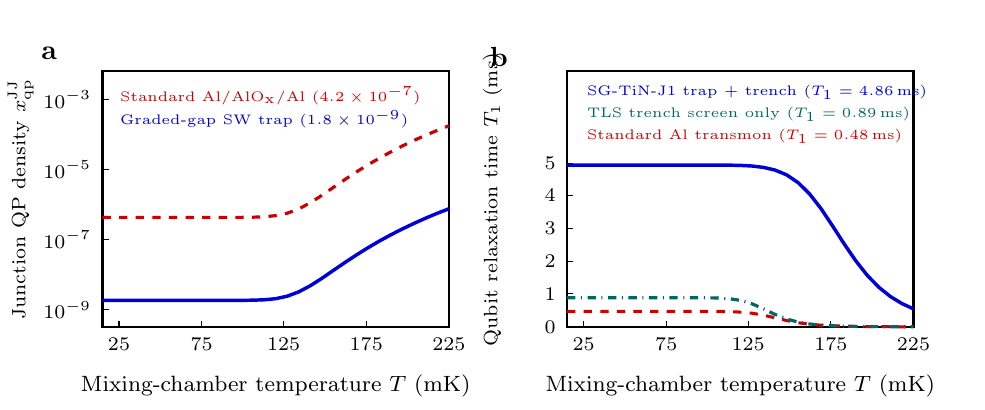
\begin{tikzpicture}[x=1cm,y=1cm]
  \useasboundingbox (0,0) rectangle (11.8,4.5);

  % Panel a: Non-Equilibrium Quasiparticle Density log10(x_qp) vs T
  \node[anchor=north west,font=\bfseries\normalsize] at (0.05,4.38) {a};
  \draw[thick] (0.95,0.70) rectangle (5.35,3.95);
  \foreach \v/\y in {-9/0.92, -7/1.81, -5/2.70, -3/3.59} {
    \draw (0.95,\y) -- (1.03,\y);
    \node[left,font=\scriptsize] at (0.93,\y) {$10^{\v}$};
  }
  \foreach \xval/\xpos in {25/1.16, 75/2.21, 125/3.25, 175/4.30, 225/5.35} {
    \draw (\xpos,0.70) -- (\xpos,0.78);
    \node[below,font=\scriptsize] at (\xpos,0.68) {\xval};
  }
  \node[below,font=\footnotesize] at (3.15,0.22) {Mixing-chamber temperature $T$ ($\mathrm{mK}$)};
  \node[rotate=90,above,font=\scriptsize] at (0.20,2.32) {Junction QP density $x_{\mathrm{qp}}^{\mathrm{JJ}}$};

  \draw[red!80!black,dashed,line width=1.15pt] (0.950,2.091) -- (1.097,2.091) -- (1.243,2.091) -- (1.390,2.091) -- (1.537,2.091) -- (1.683,2.091) -- (1.830,2.091) -- (1.977,2.091) -- (2.123,2.091) -- (2.270,2.091) -- (2.417,2.091) -- (2.563,2.091) -- (2.710,2.091) -- (2.857,2.093) -- (3.003,2.098) -- (3.150,2.113) -- (3.297,2.144) -- (3.443,2.198) -- (3.590,2.277) -- (3.737,2.371) -- (3.883,2.472) -- (4.030,2.572) -- (4.177,2.669) -- (4.323,2.760) -- (4.470,2.845) -- (4.617,2.925) -- (4.763,3.000) -- (4.910,3.070) -- (5.057,3.135) -- (5.203,3.196) -- (5.350,3.254);
  \draw[blue!85!black,line width=1.25pt] (0.950,1.036) -- (1.097,1.036) -- (1.243,1.036) -- (1.390,1.036) -- (1.537,1.036) -- (1.683,1.036) -- (1.830,1.036) -- (1.977,1.036) -- (2.123,1.036) -- (2.270,1.036) -- (2.417,1.036) -- (2.563,1.036) -- (2.710,1.037) -- (2.857,1.039) -- (3.003,1.044) -- (3.150,1.058) -- (3.297,1.090) -- (3.443,1.145) -- (3.590,1.223) -- (3.737,1.317) -- (3.883,1.418) -- (4.030,1.518) -- (4.177,1.615) -- (4.323,1.706) -- (4.470,1.792) -- (4.617,1.872) -- (4.763,1.946) -- (4.910,2.016) -- (5.057,2.082) -- (5.203,2.143) -- (5.350,2.200);

  \node[anchor=north west,font=\tiny,red!80!black] at (1.05,3.88) {Standard $\mathrm{Al/AlO_x/Al}$ ($4.2\times 10^{-7}$)};
  \node[anchor=north west,font=\tiny,blue!85!black] at (1.05,3.58) {Graded-gap SW trap ($1.8\times 10^{-9}$)};

  % Panel b: Superconducting Qubit Relaxation Time T1 vs Temperature
  \node[anchor=north west,font=\bfseries\normalsize] at (5.75,4.38) {b};
  \draw[thick] (6.85,0.70) rectangle (11.25,3.95);
  \foreach \v/\y in {0/0.70, 1/1.12, 2/1.53, 3/1.95, 4/2.37, 5/2.78} {
    \draw (6.85,\y) -- (6.93,\y);
    \node[left,font=\scriptsize] at (6.83,\y) {\v};
  }
  \foreach \xval/\xpos in {25/7.06, 75/8.11, 125/9.15, 175/10.20, 225/11.25} {
    \draw (\xpos,0.70) -- (\xpos,0.78);
    \node[below,font=\scriptsize] at (\xpos,0.68) {\xval};
  }
  \node[below,font=\footnotesize] at (9.05,0.22) {Mixing-chamber temperature $T$ ($\mathrm{mK}$)};
  \node[rotate=90,above,font=\scriptsize] at (6.15,2.32) {Qubit relaxation time $T_1$ ($\mathrm{ms}$)};

  \draw[red!80!black,dashed,line width=1.1pt] (6.850,0.898) -- (6.997,0.898) -- (7.143,0.898) -- (7.290,0.898) -- (7.437,0.898) -- (7.583,0.898) -- (7.730,0.898) -- (7.877,0.898) -- (8.023,0.898) -- (8.170,0.898) -- (8.317,0.898) -- (8.463,0.898) -- (8.610,0.898) -- (8.757,0.897) -- (8.903,0.894) -- (9.050,0.888) -- (9.197,0.874) -- (9.343,0.849) -- (9.490,0.816) -- (9.637,0.781) -- (9.783,0.753) -- (9.930,0.734) -- (10.077,0.721) -- (10.223,0.714) -- (10.370,0.709) -- (10.517,0.706) -- (10.663,0.704) -- (10.810,0.703) -- (10.957,0.702) -- (11.103,0.701) -- (11.250,0.701);
  \draw[teal!80!black,dashdotted,line width=1.15pt] (6.850,1.071) -- (6.997,1.071) -- (7.143,1.071) -- (7.290,1.071) -- (7.437,1.071) -- (7.583,1.071) -- (7.730,1.071) -- (7.877,1.071) -- (8.023,1.071) -- (8.170,1.071) -- (8.317,1.071) -- (8.463,1.071) -- (8.610,1.070) -- (8.757,1.067) -- (8.903,1.059) -- (9.050,1.037) -- (9.197,0.994) -- (9.343,0.930) -- (9.490,0.859) -- (9.637,0.801) -- (9.783,0.761) -- (9.930,0.737) -- (10.077,0.722) -- (10.223,0.714) -- (10.370,0.709) -- (10.517,0.706) -- (10.663,0.704) -- (10.810,0.703) -- (10.957,0.702) -- (11.103,0.701) -- (11.250,0.701);
  \draw[blue!85!black,line width=1.25pt] (6.850,2.755) -- (6.997,2.755) -- (7.143,2.755) -- (7.290,2.755) -- (7.437,2.755) -- (7.583,2.755) -- (7.730,2.755) -- (7.877,2.755) -- (8.023,2.755) -- (8.170,2.755) -- (8.317,2.755) -- (8.463,2.755) -- (8.610,2.755) -- (8.757,2.755) -- (8.903,2.754) -- (9.050,2.751) -- (9.197,2.743) -- (9.343,2.726) -- (9.490,2.692) -- (9.637,2.632) -- (9.783,2.533) -- (9.930,2.389) -- (10.077,2.200) -- (10.223,1.981) -- (10.370,1.753) -- (10.517,1.539) -- (10.663,1.354) -- (10.810,1.203) -- (10.957,1.085) -- (11.103,0.996) -- (11.250,0.928);

  \node[anchor=north west,font=\tiny,blue!85!black] at (6.98,3.90) {SG-TiN-J1 trap + trench ($T_1=4.86\,\mathrm{ms}$)};
  \node[anchor=north west,font=\tiny,teal!80!black] at (6.98,3.62) {TLS trench screen only ($T_1=0.89\,\mathrm{ms}$)};
  \node[anchor=north west,font=\tiny,red!80!black] at (6.98,3.34) {Standard $\mathrm{Al}$ transmon ($T_1=0.48\,\mathrm{ms}$)};
\end{tikzpicture}
